
\item A round cone with half-angle \( \alpha = 30^\circ \) and the radius of the base \( R = 5.0 \) cm rolls uniformly and without slipping over a horizontal plane as shown in Fig. 1.8. The cone apex is hinged at the point \( O \) which is on the same level with the point \( C \), the cone base centre. The velocity of point \( C \) is \( v = 10.0 \) cm/s. Find the moduli of
\begin{center}
    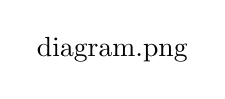
\begin{tikzpicture}
        \node at (0, 0) {diagram.png};
    \end{tikzpicture}
\end{center}
\begin{enumerate}
    \item the vector of the angular velocity of the cone and the angle it forms with the vertical;
    \item the vector of the angular acceleration of the cone.
\end{enumerate}